% Provenance (never printed): cycle 4 SVT, "La planete Terre": the dynamics of
% the Earth's outer shell, plates and their boundaries, continental drift as a
% history of ideas; see sources/outline_sources.md. Pilot chapter, 2026-10-22.
\chapter{تكتونية الصفائح: الأحجية المتحركة}\label{ch:g7:plate-tectonics}

افرد \omterm{def:g3:continents-and-oceans:world-map}{خريطة للعالم} على طاولة وانظر إلى شاطئي \omterm{def:g2:water-on-earth:ocean}{المحيط}
الأطلسي. فالانتفاخ الكبير للبرازيل يبدو كأنه صُنع لينزلق في
تجويف \omterm{def:g1:landscapes-around-us:water}{الساحل} الغربي لإفريقيا، كأن أحدًا قطع قطعة واحدة من
اليابسة نصفين ثم أبعد النصفين أحدهما عن الآخر. وقد لاحظ ذلك أول من طبعوا خرائط
جيدة للساحلين على الفور. وظل الأمر طرفة غريبة ثلاثة قرون. ثم صار
في القرن العشرين نقطة انطلاق النظرية التي تفسر اليوم لماذا تهتز الأرض في اليابان، ولماذا ترتفع \omterm{def:g1:landscapes-around-us:landform}{جبال} الأنديز
كل هذا الارتفاع، ولماذا تتسع آيسلندا ببطء --- ولماذا ليست \omterm{def:g2:drawing-to-map:map}{الخريطة} التي على
الطاولة إلا لقطة لعالم يتحرك.

\begin{omfigure}
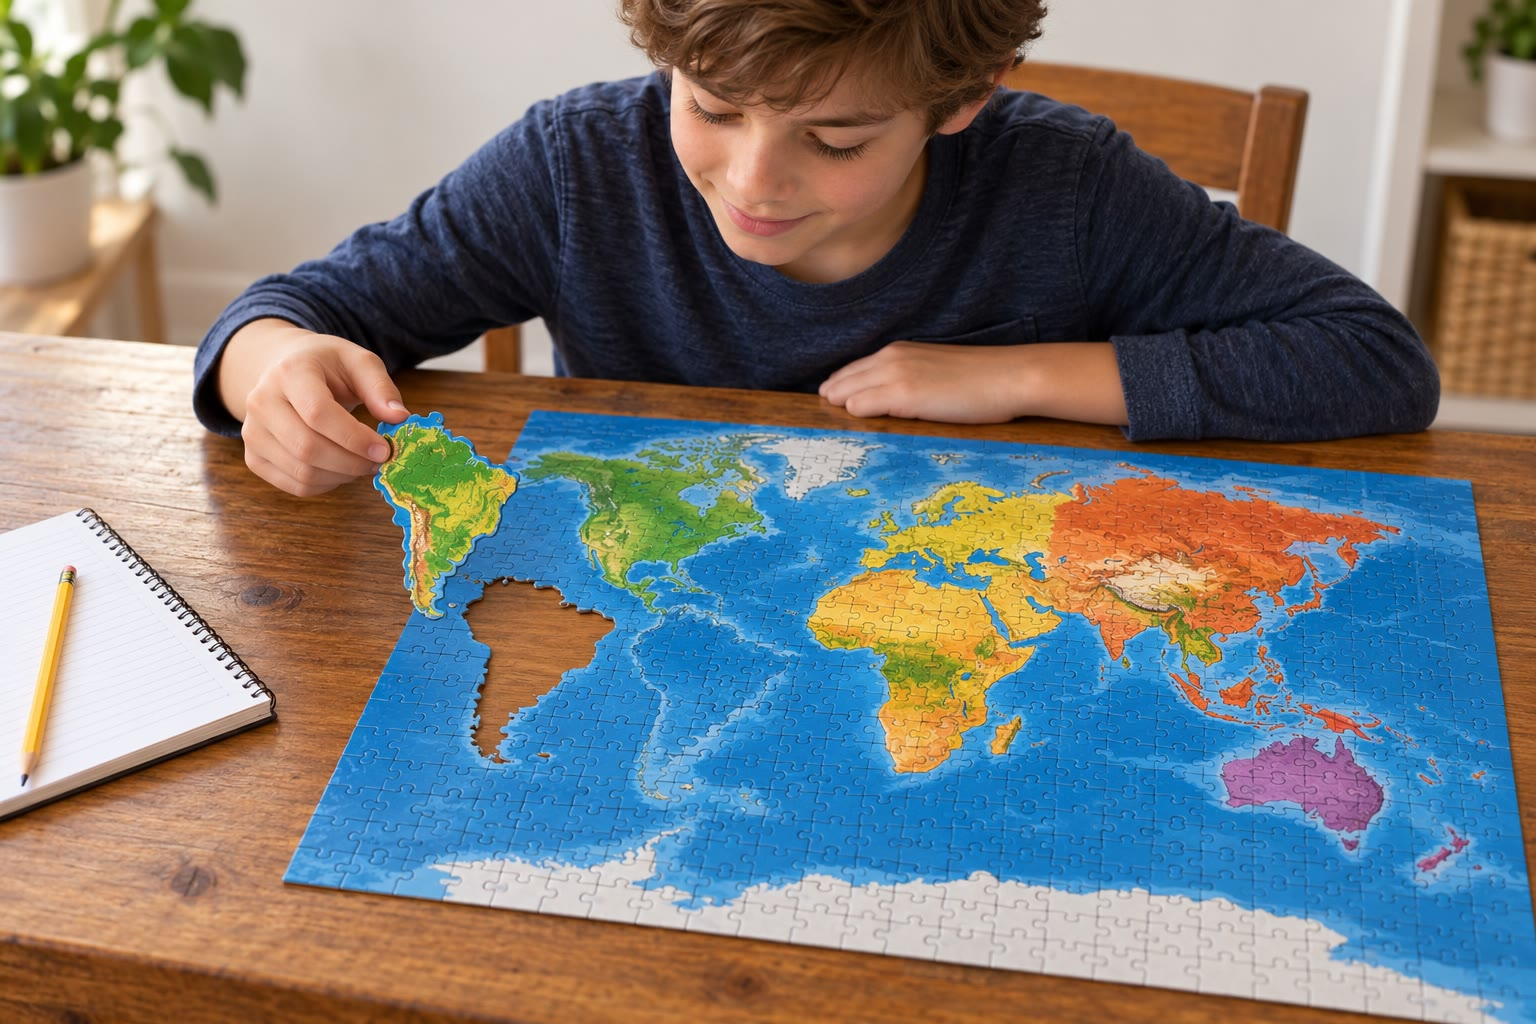
\includegraphics[width=0.62\linewidth]{images/book1/ai/g7-puzzle-map.jpg}

{\small أمريكا الجنوبية بجانب إفريقيا: في الأحجية، التطابق لعبة؛ وعلى
الأرض الحقيقية، هو دليل.}
\end{omfigure}

\begin{recall}
للأرض ثلاث طبقات رئيسية: \emph{\omterm{def:g6:inside-the-earth:layers}{قشرة}} رقيقة صخرية، و\emph{\omterm{def:g6:inside-the-earth:layers}{وشاح}}
سميك من \omterm{def:g3:stones-pebbles-sand:rock}{الصخر} الحار، و\emph{\omterm{def:g6:inside-the-earth:layers}{لب}} فلزي؛ وترتفع درجة الحرارة
كلما ازداد العمق (\cref{ch:g6:inside-the-earth}). ويُحدَّد موقع المكان على الكرة الأرضية
بعرضه الجغرافي وطوله الجغرافي (\cref{ch:g6:latitude-longitude}).
\end{recall}

\section{قارات كانت متلاصقة يومًا}

\begin{definition}[الانجراف القاري]\label{def:g7:plate-tectonics:continental-drift}
\emph{الانجراف القاري}\index{انجراف قاري} هو الفكرة القائلة إن
\omterm{def:g3:continents-and-oceans:continent}{القارات} تتحرك ببطء على سطح الأرض، فتغيّرت مواقعها، وأشكال المحيطات
التي بينها، على مر
العصور.
\end{definition}

\begin{definition}[القارة العظمى]\label{def:g7:plate-tectonics:supercontinent}
\emph{القارة العظمى}\index{قارة عظمى} كتلة يابسة واحدة مكوَّنة من
كل \omterm{def:g3:continents-and-oceans:continent}{القارات}، أو من معظمها، ملتحمة معًا. وآخرها،
\emph{بانجيا}\index{بانجيا} («كل الأراضي» باليونانية)، بدأت تتفكك
قبل ما بين نحو 225 و200 مليون سنة.
% ledger: usgs:pangaea-breakup
\end{definition}

العالِم الذي دافع عن \omterm{def:g7:plate-tectonics:continental-drift}{الانجراف القاري} بوصفه نظرية حقيقية، بالأدلة،
هو ألفريد فيغنر. وقد جمع أربعة أنواع من الأدلة.

\begin{enumerate}
  \item \textbf{أشكال \omterm{def:g1:landscapes-around-us:water}{السواحل}.} تتطابق أمريكا الجنوبية وإفريقيا
        كقطعتين من لعبة التركيب، وكذلك عدة \omterm{def:g1:landscapes-around-us:water}{سواحل}
        أخرى.
  \item \textbf{الأحافير.} توجد أحافير الحيوانات والنباتات نفسها على
        \omterm{def:g3:continents-and-oceans:continent}{قارات} تفصل بينها اليوم آلاف الكيلومترات من
        \omterm{def:g2:water-on-earth:ocean}{المحيط}. و\emph{الميزوسور} زاحف صغير عاش في \omterm{def:g2:water-on-earth:salt-fresh}{الماء
        العذب}: ما كان ليستطيع أن يسبح عبر \omterm{def:g2:water-on-earth:ocean}{محيط}، ومع ذلك توجد أحافيره
        في البرازيل وفي جنوب إفريقيا معًا.
  \item \textbf{\omterm{def:g3:stones-pebbles-sand:rock}{الصخور}.} \omterm{def:g3:stones-pebbles-sand:rock}{صخور} من الأنواع والأعمار نفسها، \omterm{def:g4:world-physical-map:range}{وسلاسل جبلية}
        قديمة لها الشكل نفسه، تتوقف عند \omterm{def:g1:landscapes-around-us:water}{ساحل} ثم تبدأ من جديد على
        \omterm{def:g1:landscapes-around-us:water}{الساحل} المقابل، كما تفعل سطور جريدة ممزقة.
  \item \textbf{المناخات القديمة.} الفحم، المتكوّن من نباتات غابات
        دافئة مستنقعية، يوجد في القارة القطبية الجنوبية؛ وآثار تركتها
        \omterm{def:g1:landscapes-around-us:water}{أنهار} جليدية قديمة توجد في أجزاء من إفريقيا حارة جافة اليوم.
        فلا بد أن هذه الأراضي كانت يومًا في مناخات أخرى، وعند \omterm{def:g6:latitude-longitude:latitude}{دوائر
        عرض} أخرى.
\end{enumerate}
% ledger: usgs:coal-antarctica, usgs:fossil-map

\begin{omfigure}
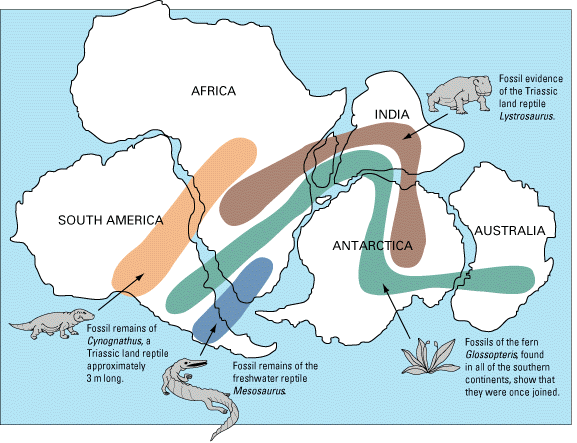
\includegraphics[width=0.86\linewidth]{images/book1/g7-usgs-fossil-map.png}

{\small \omterm{def:g3:continents-and-oceans:continent}{القارات} الجنوبية وقد أعيد جمعها. كل شريط ملوّن يصل
الأماكن التي يوجد فيها اليوم نوع واحد من الأحافير: الزاحفان البريان
\emph{الكينوغناثوس} و\emph{الليستروسورس}، والزاحف المائي العذب
\emph{الميزوسور} والسرخس \emph{الغلوسوبتيريس}. حين تكون \omterm{def:g3:continents-and-oceans:continent}{القارات}
منفصلة تتبعثر الأشرطة؛ وحين تلتحم، تمتد الأشرطة دون انقطاع.
\omterm{def:g2:drawing-to-map:map}{الخريطة}: هيئة المسح الجيولوجي الأمريكية، \emph{هذه الأرض الديناميكية} (ملك عام).}
\end{omfigure}

\begin{history}[فكرة فيغنر، 1912--1930]
% ledger: usgs:wegener-1912, usgs:wegener-death, usgs:jeffreys
عرض ألفريد فيغنر، وهو عالم أرصاد جوية ألماني في الثانية والثلاثين، نظرية
\omterm{def:g7:plate-tectonics:continental-drift}{الانجراف القاري} في مقالين عام 1912. ورفضها معظم الجيولوجيين.
وكان أقوى اعتراض أن فيغنر لم يستطع أن يقول \emph{ما الذي} يحرك
\omterm{def:g3:continents-and-oceans:continent}{القارات}: فقد ظن أنها تشق طريقها عبر \omterm{def:g3:stones-pebbles-sand:rock}{صخر} قاع
\omterm{def:g2:water-on-earth:ocean}{المحيط}، وبيّن الفيزيائي هارولد جيفريز أن \omterm{def:g3:continents-and-oceans:continent}{القارات} الصلبة لا يمكن
أن تفعل ذلك دون أن تتحطم. وظل فيغنر يجمع الأدلة حتى
مات على الغطاء الجليدي لغرينلاند عام 1930، أثناء بعثة. والجواب
الذي كان ينقصه جاء من قيعان المحيطات، التي استُكشفت بعد خمسينيات القرن العشرين: وهو
يُروى في سنة لاحقة.
\end{history}

\section{الصفائح}

كانت أدلة فيغنر صحيحة، لكن قاراته لم تكن القطع الصحيحة. فليست
\omterm{def:g3:continents-and-oceans:continent}{القارات} وحدها هي التي تتحرك: بل الغلاف الخارجي للأرض كله،
تحت \omterm{def:g3:continents-and-oceans:continent}{القارات} وتحت المحيطات على السواء، مكسَّر قطعًا.

\begin{definition}[الصفيحة التكتونية]\label{def:g7:plate-tectonics:plate}
\emph{الصفيحة التكتونية}\index{صفيحة تكتونية} (أو الصفيحة اختصارًا)
لوح صخري كبير صلب يشكّل جزءًا من الغلاف الخارجي للأرض.
وتتكون الصفيحة من \omterm{def:g6:inside-the-earth:layers}{القشرة} ومن الجزء العلوي البارد الصلب من
\omterm{def:g6:inside-the-earth:layers}{الوشاح}، ويبلغ سمكهما معًا 80 كيلومترًا على الأقل في المتوسط؛ وهي تتحرك ببطء
فوق \omterm{def:g6:inside-the-earth:layers}{الوشاح} الأشد حرارة والأطرى الذي تحتها.
% ledger: usgs:lithosphere-80km
\end{definition}

\begin{definition}[تكتونية الصفائح]\label{def:g7:plate-tectonics:plate-tectonics}
\emph{تكتونية الصفائح}\index{تكتونية الصفائح} هي النظرية القائلة إن الغلاف
الخارجي للأرض مقسَّم إلى \omterm{def:g7:plate-tectonics:plate}{صفائح} يتحرك بعضها بالنسبة إلى
بعض، وإن معظم \omterm{def:g4:volcanoes-earthquakes-first-look:earthquake}{الزلازل} \omterm{def:g4:volcanoes-earthquakes-first-look:volcano}{والبراكين} \omterm{def:g4:world-physical-map:range}{والسلاسل الجبلية}
تنشأ حيث تلتقي \omterm{def:g7:plate-tectonics:plate}{الصفائح}.
\end{definition}

\begin{remark}[كم عدد الصفائح؟]\label{rem:g7:plate-tectonics:how-many}
% ledger: usgs:plates-dozen, pb2002:count
نحو اثنتي عشرة \omterm{def:g7:plate-tectonics:plate}{صفيحة} كبيرة؛ والصغيرة أكثر بكثير. \omterm{def:g2:drawing-to-map:map}{وخريطة} مفصلة يستعملها
الجيولوجيون تحصي 52 \omterm{def:g7:plate-tectonics:plate}{صفيحة}. وقد تحمل \omterm{def:g7:plate-tectonics:plate}{الصفيحة} \omterm{def:g3:continents-and-oceans:continent}{قارة}، أو محيطًا، أو
الاثنين معًا: \omterm{def:g7:plate-tectonics:plate}{فصفيحة} أمريكا الجنوبية تحمل أمريكا الجنوبية كلها
والنصف الغربي من جنوب \omterm{def:g2:water-on-earth:ocean}{المحيط} الأطلسي. أما \omterm{def:g7:plate-tectonics:plate}{صفيحة} \omterm{def:g2:water-on-earth:ocean}{المحيط} الهادئ، وهي أكبرها،
فتكاد لا تحمل أي يابسة.
\end{remark}

\begin{omfigure}
\begin{tikzpicture}
\begin{axis}[ommap, width=\linewidth, xtick={-180,-90,...,180}, ytick={-60,0,60}]
\addplot[fill=omLithAlluv, draw=black!45, line width=0.2pt] table {figdata/out/shared-geo-land.dat};
\addplot[omRidge, line width=0.8pt] table {figdata/out/shared-geo-school-ridge.dat};
\addplot[omRidge!70!black, line width=0.8pt] table {figdata/out/shared-geo-school-transform.dat};
\addplot[omTrench, line width=0.8pt] table {figdata/out/shared-geo-school-subduction.dat};
\addplot[fill=omTrench, draw=none] table {figdata/out/shared-geo-school-teeth.dat};
\addplot[black!65, line width=0.8pt] table {figdata/out/shared-geo-school-collision.dat};
\begin{scope}[every node/.style={font=\scriptsize\bfseries, text=black!85,
    fill=white, fill opacity=0.75, text opacity=1, inner sep=1pt, align=center}]
  \node at (axis cs:-150,12) {الهادئ};
  \node at (axis cs:-103,52) {أمريكا\\الشمالية};
  \node at (axis cs:-48,-12) {أمريكا\\الجنوبية};
  \node at (axis cs:85,57) {الأوراسية};
  \node at (axis cs:18,8) {الإفريقية};
  \node at (axis cs:10,-75) {القطبية الجنوبية};
  \node at (axis cs:78,11) {الهندية};
  \node at (axis cs:128,-26) {الأسترالية};
  \node at (axis cs:-95,-22) {نازكا};
  \node at (axis cs:50,20) {العربية};
\end{scope}
\end{axis}
\end{tikzpicture}

{\small \omterm{def:g7:plate-tectonics:plate}{الصفائح} التكتونية الرئيسية. الأحمر: \omterm{def:g7:plate-tectonics:plate}{صفائح} تتباعد؛ الأزرق ذو
المثلثات: \omterm{def:g7:plate-tectonics:plate}{صفيحة} تغوص تحت الأخرى (المثلثات على
\omterm{def:g7:plate-tectonics:plate}{الصفيحة} التي تبقى في الأعلى)؛ الرمادي: \omterm{def:g7:plate-tectonics:plate}{صفائح} تتدافع عبر نطاق عريض
من \omterm{def:g1:landscapes-around-us:landform}{الجبال}؛ الأحمر الداكن: \omterm{def:g7:plate-tectonics:plate}{صفائح} تنزلق إحداها بمحاذاة الأخرى. الحدود بحسب
ب.~بيرد (2003)؛ \omterm{def:g1:landscapes-around-us:water}{والسواحل} من Natural Earth.}
\end{omfigure}

كيف نعرف أين تنتهي \omterm{def:g7:plate-tectonics:plate}{صفيحة} وأين تبدأ التالية؟ انظر إلى حيث تكون
الأرض مضطربة.

\begin{proposition}[الزلازل والبراكين ترسم حدود الصفائح]\label{prop:g7:plate-tectonics:restless}
% ledger: data:usgs-comcat, data:pb2002 (share computed in figdata/grade-7/quakes_on_boundaries.py)
\omterm{def:g4:volcanoes-earthquakes-first-look:earthquake}{الزلازل} \omterm{def:g4:volcanoes-earthquakes-first-look:volcano}{والبراكين} ليست مبعثرة عشوائيًا على الأرض: فمعظمها
يقع على طول أحزمة ضيقة، وهذه الأحزمة هي حواف
\omterm{def:g7:plate-tectonics:plate}{الصفائح}. فمن بين \omterm{def:g4:volcanoes-earthquakes-first-look:earthquake}{الزلازل} التي بلغت قوتها 6 درجات أو أكثر وسُجّلت بين
1976 و2025، وعددها 7\,031، وقع 6\,472 --- أي 92\,\% --- على بعد أقل من
\qty{300}{km} من \omterm{def:g7:plate-tectonics:plate-boundary}{حد صفائح}.
\end{proposition}

\begin{omfigure}
\begin{tikzpicture}
\begin{axis}[ommap, width=\linewidth, xtick={-180,-90,...,180}, ytick={-60,0,60},
  legend style={at={(0.02,0.04)}, anchor=south west, font=\scriptsize,
  fill=white, fill opacity=0.85, text opacity=1, draw=black!40}]
\addplot[fill=omLithAlluv, draw=black!45, line width=0.2pt, forget plot] table {figdata/out/shared-geo-land.dat};
\addplot[only marks, mark=*, mark size=0.45pt, omThm!85!black] table[x=lon, y=lat] {figdata/out/grade-7-quakes_on_boundaries-map.dat};
\addlegendentry{\foreignlanguage{arabic}{زلزال قوته \babelsublr{6.5} أو أكثر، بين \babelsublr{1976} و\babelsublr{2025}}}
\addplot[only marks, mark=triangle*, mark size=1.1pt, black] table {figdata/out/shared-geo-volcanoes.dat};
\addlegendentry{\foreignlanguage{arabic}{بركان نشط في آخر \babelsublr{12\,000} سنة}}
\end{axis}
\end{tikzpicture}

{\small \omterm{def:g4:volcanoes-earthquakes-first-look:earthquake}{الزلازل} الكبيرة \omterm{def:g4:volcanoes-earthquakes-first-look:volcano}{والبراكين} الحديثة. قارنها \omterm{def:g2:drawing-to-map:map}{بخريطة}
\omterm{def:g7:plate-tectonics:plate}{الصفائح} أعلاه: النقاط والمثلثات ترسم \omterm{def:g7:plate-tectonics:plate-boundary}{حدود الصفائح}. البيانات:
فهرس \omterm{def:g4:volcanoes-earthquakes-first-look:earthquake}{الزلازل} لهيئة المسح الجيولوجي الأمريكية؛ وبرنامج \omterm{def:g4:volcanoes-earthquakes-first-look:volcano}{البراكين} العالمي
التابع لمؤسسة سميثسونيان.}
\end{omfigure}

\section{ثلاثة أنواع من حدود الصفائح}

\begin{definition}[حد الصفائح]\label{def:g7:plate-tectonics:plate-boundary}
\emph{حد الصفائح}\index{حد الصفائح} هو الخط، أو النطاق
الضيق، الذي تلتقي عنده صفيحتان. وبحسب الطريقة التي تتحرك بها الصفيحتان
إحداهما بالنسبة إلى الأخرى، يكون الحد من أحد ثلاثة أنواع:
\begin{itemize}
  \item عند \emph{الحد المتباعد}\index{حد متباعد} تبتعد
        الصفيحتان إحداهما عن الأخرى؛
  \item عند \emph{الحد المتقارب}\index{حد متقارب} تقترب
        الصفيحتان إحداهما من الأخرى؛
  \item عند \emph{الحد التحويلي}\index{حد تحويلي} تنزلق
        الصفيحتان إحداهما بمحاذاة الأخرى، جنبًا إلى جنب.
\end{itemize}
\end{definition}

\begin{example}[حدود متباعدة: آيسلندا وشرق إفريقيا]\label{ex:g7:plate-tectonics:divergent}
% ledger: usgs:iceland, usgs:east-africa
في وسط \omterm{def:g2:water-on-earth:ocean}{المحيط} الأطلسي تمتد سلسلة من \omterm{def:g1:landscapes-around-us:landform}{الجبال} المغمورة،
هي ظهرة وسط الأطلسي، حيث تتباعد الصفيحتان الواقعتان على جانبيها. فيصعد \omterm{def:g3:stones-pebbles-sand:rock}{صخر}
حار من \omterm{def:g6:inside-the-earth:layers}{الوشاح} إلى الفجوة، وينصهر جزئيًا، ويصير قاعًا جديدًا
\omterm{def:g2:water-on-earth:ocean}{للبحر}: \omterm{def:g7:plate-tectonics:plate-boundary}{فالحد المتباعد} يبني \omterm{def:g7:plate-tectonics:plate}{صفيحة} جديدة. وآيسلندا قطعة من
هذه الظهرة ترتفع فوق \omterm{def:g2:water-on-earth:ocean}{البحر}: وهناك، تتحرك أمريكا الشمالية نحو الغرب
وأوراسيا نحو الشرق، فتتمزق الجزيرة ببطء. وبين عامي 1975
و1984، اتسعت الشقوق القريبة من \omterm{def:g4:volcanoes-earthquakes-first-look:volcano}{بركان} كرافلا، في شمال الجزيرة،
بنحو 7 أمتار في المجموع. ويمكن \omterm{def:g7:plate-tectonics:plate-boundary}{للحد المتباعد} أيضًا أن يشق
\omterm{def:g3:continents-and-oceans:continent}{قارة}: فعلى طول أخدود شرق إفريقيا، بدأت إفريقيا تنقسم،
\omterm{def:g2:water-on-earth:ocean}{والبحر} الأحمر \omterm{def:g2:water-on-earth:ocean}{محيط} فتي فصل الجزيرة العربية عن
إفريقيا من قبل.
\end{example}

\begin{example}[حدود متقاربة: الأنديز والهيمالايا]\label{ex:g7:plate-tectonics:convergent}
% ledger: usgs:trench-depth, usgs:himalaya
قبالة \omterm{def:g1:landscapes-around-us:water}{الساحل} الغربي لأمريكا الجنوبية، تتحرك \omterm{def:g7:plate-tectonics:plate}{صفيحة} نازكا، التي تحمل محيطًا،
نحو \omterm{def:g7:plate-tectonics:plate}{صفيحة} أمريكا الجنوبية، التي تحمل \omterm{def:g3:continents-and-oceans:continent}{قارة}. فتنثني
\omterm{def:g7:plate-tectonics:plate}{الصفيحة} المحيطية، وهي الأثقل، وتغوص تحت \omterm{def:g3:continents-and-oceans:continent}{القارة}، عميقًا في
\omterm{def:g6:inside-the-earth:layers}{الوشاح}. وعلى طول الخط الذي تنزل عنده، ينحدر قاع \omterm{def:g2:water-on-earth:ocean}{البحر} في
خندق عميق؛ وفوق \omterm{def:g7:plate-tectonics:plate}{الصفيحة} الغائصة، تهز \omterm{def:g4:volcanoes-earthquakes-first-look:earthquake}{الزلازل} اليابسة
وتصطف عليها \omterm{def:g4:volcanoes-earthquakes-first-look:volcano}{البراكين}: إنها \omterm{def:g1:landscapes-around-us:landform}{جبال} الأنديز. وفي غرب \omterm{def:g2:water-on-earth:ocean}{المحيط} الهادئ، حيث تغوص \omterm{def:g7:plate-tectonics:plate}{صفيحة} محيطية
تحت أخرى، تكون الخنادق أعمق الأماكن على الأرض:
فعمق خندق ماريانا يقارب \qty{11000}{m}. وحين تلتقي قارتان،
لا تغوص أي منهما: بل تتجعد \omterm{def:g6:inside-the-earth:layers}{القشرة} وتزداد سمكًا. وقد اصطدمت الهند بآسيا
قبل نحو 50 مليون سنة، ولا تزال الصفيحتان تتدافعان؛ وهكذا
ارتفعت \omterm{def:g1:landscapes-around-us:landform}{جبال} الهيمالايا وهضبة التبت.
\end{example}

\begin{example}[حد تحويلي: صدع سان أندرياس]\label{ex:g7:plate-tectonics:transform}
% ledger: usgs:san-andreas, usgs:san-andreas-photo
في كاليفورنيا، تنزلق \omterm{def:g7:plate-tectonics:plate}{صفيحة} \omterm{def:g2:water-on-earth:ocean}{المحيط} الهادئ نحو الشمال الغربي بمحاذاة \omterm{def:g7:plate-tectonics:plate}{صفيحة}
أمريكا الشمالية على طول صدع سان أندرياس، الذي يبلغ طوله نحو \qty{1300}{km}. ولا
تُصنع هناك \omterm{def:g7:plate-tectonics:plate}{صفيحة} ولا تُدمَّر؛ بل تحتك الصفيحتان إحداهما بالأخرى،
وهزات ذلك الاحتكاك هي \omterm{def:g4:volcanoes-earthquakes-first-look:earthquake}{الزلازل}.
\end{example}

\begin{omfigure}
\begin{tikzpicture}[x=1cm, y=1cm, font=\small]
  % mantle
  \fill[omLithGranite!45] (0,-3.3) rectangle (12.4,-0.85);
  \node[font=\footnotesize, text=black!75] at (2.6,-2.6) {الوشاح: حار وطري};
  % sea water
  \fill[omSea] (0,0) -- (0,-0.75) -- (1.5,-0.6) -- (3,-0.25) -- (4.5,-0.6)
    -- (7.4,-0.8) -- (8.0,-1.2) -- (8.6,-0.6) -- (8.9,0) -- cycle;
  % oceanic plates (the ridge at x = 3, the trench at x = 8)
  \fill[omLithBasalt!70] (0,-0.75) -- (1.5,-0.6) -- (3,-0.25) -- (4.5,-0.6)
    -- (7.4,-0.8) -- (8.0,-1.2) -- (9.6,-2.3) -- (10.2,-3.3) -- (9.5,-3.3)
    -- (8.6,-2.2) -- (7.5,-1.55) -- (4.5,-1.35) -- (3.2,-0.95) -- (2.8,-0.95)
    -- (1.5,-1.35) -- (0,-1.45) -- cycle;
  % continental plate
  \fill[omLithSand!80] (8.6,-0.6) -- (8.9,0) -- (9.4,0.35) -- (9.8,0.9)
    -- (10.2,0.35) -- (12.4,0.2) -- (12.4,-1.9) -- (10.6,-1.9) -- (9.6,-2.3)
    -- (8.0,-1.2) -- cycle;
  \draw[black!70, line width=0.5pt] (0,-0.75) -- (1.5,-0.6) -- (3,-0.25)
    -- (4.5,-0.6) -- (7.4,-0.8) -- (8.0,-1.2) -- (8.6,-0.6) -- (8.9,0)
    -- (9.4,0.35) -- (9.8,0.9) -- (10.2,0.35) -- (12.4,0.2);
  \draw[black!45, densely dashed] (0,0) -- (8.9,0);
  % magma: under the ridge and under the volcano
  \fill[omThm!80] (2.85,-0.95) -- (3,-0.3) -- (3.15,-0.95) -- cycle;
  \draw[omThm!80, line width=1.4pt, -{Stealth[length=2.2mm]}] (3,-1.85) -- (3,-1.0);
  \draw[omThm!80, line width=1.2pt, decorate, decoration={snake, amplitude=0.6pt,
    segment length=4pt}] (9.8,-2.45) -- (9.8,0.75);
  % plate motions
  \draw[black, line width=1pt, -{Stealth[length=2.4mm]}] (2.5,-0.75) -- (1.3,-0.95);
  \draw[black, line width=1pt, -{Stealth[length=2.4mm]}] (3.5,-0.75) -- (5.4,-1.05);
  \draw[black, line width=1pt, -{Stealth[length=2.4mm]}] (12.1,-0.85) -- (10.9,-0.85);
  \draw[black, line width=1pt, -{Stealth[length=2.4mm]}] (8.7,-1.75) -- (9.3,-2.25);
  % labels
  \node[font=\footnotesize, align=center, above] at (3,0.05) {حد متباعد\\ظهرة محيطية};
  \node[font=\footnotesize, align=center, below] at (6.9,-1.95) {حد متقارب\\الصفيحة المحيطية تغوص};
  \draw[black!60, thin] (8.0,-1.25) -- (7.6,-1.9);
  \node[font=\footnotesize, above] at (8.0,0.05) {خندق};
  \draw[black!60, thin] (8.0,0.05) -- (8.0,-1.1);
  \node[font=\footnotesize, above] at (9.8,0.95) {بركان};
  \node[font=\footnotesize] at (11.4,-0.4) {قارة};
  \node[font=\footnotesize] at (1.2,-1.6) {صفيحة محيطية};
  \node[font=\footnotesize, text=black!70] at (5.6,-0.32) {محيط};
\end{tikzpicture}

\medskip
\begin{tikzpicture}[font=\small]
  \fill[omLithBasalt!45] (0,0) rectangle (2.4,2.2);
  \fill[omLithSand!70] (2.4,0) rectangle (4.8,2.2);
  \draw[fault] (2.4,-0.1) -- (2.4,2.3);
  \draw[black, line width=1pt, -{Stealth[length=2.4mm]}] (1.2,0.5) -- (1.2,1.7);
  \draw[black, line width=1pt, -{Stealth[length=2.4mm]}] (3.6,1.7) -- (3.6,0.5);
  \node[font=\footnotesize, below] at (1.2,-0.1) {\foreignlanguage{arabic}{الصفيحة A}};
  \node[font=\footnotesize, below] at (3.6,-0.1) {\foreignlanguage{arabic}{الصفيحة B}};
  \node[font=\footnotesize, align=left, anchor=west] at (5.1,1.1)
    {حد تحويلي، كما يُرى من فوق\\الصفيحتان تنزلقان إحداهما بمحاذاة الأخرى\\لا تُصنع صفيحة ولا تُدمَّر};
\end{tikzpicture}

{\small في الأعلى: مقطع عبر حدين من \omterm{def:g7:plate-tectonics:plate-boundary}{حدود الصفائح} (بلا مقياس رسم؛ والأعماق
مضخَّمة كثيرًا). عند الظهرة تتباعد الصفيحتان ويصعد \omterm{def:g3:stones-pebbles-sand:rock}{صخر} حار
من \omterm{def:g6:inside-the-earth:layers}{الوشاح}؛ وعند الخندق تغوص \omterm{def:g7:plate-tectonics:plate}{الصفيحة} المحيطية تحت \omterm{def:g3:continents-and-oceans:continent}{القارة}،
\omterm{def:g3:stones-pebbles-sand:rock}{والصخر} الذي ينصهر فوقها يغذي \omterm{def:g4:volcanoes-earthquakes-first-look:volcano}{البراكين}. في الأسفل: \omterm{def:g7:plate-tectonics:plate-boundary}{حد
تحويلي} كما يُرى من فوق.}
\end{omfigure}

\begin{omfigure}
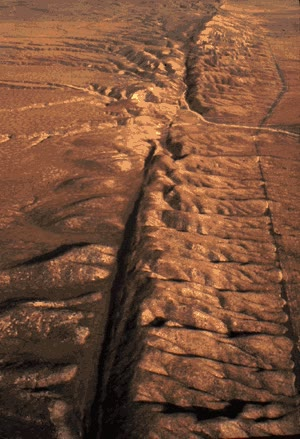
\includegraphics[width=0.28\linewidth]{images/book1/g7-usgs-san-andreas.jpg}

{\small صدع سان أندرياس يعبر \omterm{def:g1:landscapes-around-us:landform}{سهل} كاريزو، في كاليفورنيا، كما يُرى
من طائرة: \omterm{def:g1:landscapes-around-us:landform}{الوادي} المستقيم الطويل هو الحد بين
\omterm{def:g7:plate-tectonics:plate}{صفيحة} \omterm{def:g2:water-on-earth:ocean}{المحيط} الهادئ (إلى اليسار) \omterm{def:g7:plate-tectonics:plate}{وصفيحة} أمريكا الشمالية (إلى اليمين). الصورة:
روبرت إ.~والاس، هيئة المسح الجيولوجي الأمريكية (ملك عام).}
\end{omfigure}

\begin{method}[التعرف على حد صفائح على خريطة]\label{met:g7:plate-tectonics:recognise}
لتحديد نوع الحد الذي يفصل بين صفيحتين:
\begin{enumerate}
  \item ابحث، على \omterm{def:g2:drawing-to-map:map}{خريطة} لحركات \omterm{def:g7:plate-tectonics:plate}{الصفائح}، عن الأسهم الواقعة على جانبي
        الحد؛
  \item إذا كانت تشير بعيدًا عن الحد، فهو متباعد؛ وإذا كانت
        تشير نحوه، فهو متقارب؛ وإذا كانت موازية له وتشير
        في اتجاهين متعاكسين، فهو تحويلي؛
  \item تحقق بالاستعانة \omterm{def:g1:landscapes-around-us:landscape}{بالمنظر} الطبيعي: الظهرة في وسط \omterm{def:g2:water-on-earth:ocean}{محيط} أو
        الأخدود الذي يشق \omterm{def:g3:continents-and-oceans:continent}{قارة} يرافقان \omterm{def:g7:plate-tectonics:plate-boundary}{الحد المتباعد}؛ والخندق العميق
        مع خط من \omterm{def:g4:volcanoes-earthquakes-first-look:volcano}{البراكين}، أو \omterm{def:g4:world-physical-map:range}{السلسلة الجبلية} العالية، يرافقان \omterm{def:g7:plate-tectonics:plate-boundary}{الحد
        المتقارب}؛ والصدع المستقيم الطويل الذي لا يرافقه هذا ولا ذاك يرافق \omterm{def:g7:plate-tectonics:plate-boundary}{الحد
        التحويلي}.
\end{enumerate}
\end{method}

\section{ما سرعة حركة الصفائح؟}

\begin{proposition}[بضعة سنتيمترات في السنة]\label{prop:g7:plate-tectonics:speed}
% ledger: data:pb2002 (speeds computed in figdata/grade-7/plate_speeds.py), usgs:mar-rate
تتحرك صفيحتان متجاورتان إحداهما بالنسبة إلى الأخرى بسرعة بضعة
سنتيمترات في السنة: من نحو 2 سنتيمتر في السنة عبر
شمال الأطلسي إلى أكثر من 14 سنتيمترًا في السنة عبر ظهرة شرق \omterm{def:g2:water-on-earth:ocean}{المحيط}
الهادئ، وهي أسرع الظهرات اتساعًا على الأرض.
\end{proposition}

\begin{omfigure}
\begin{tikzpicture}
\begin{axis}[xbar, width=0.82\linewidth, height=5.4cm, xmin=0, xmax=16.5,
  ytick={1,...,6}, yticklabels={ظهرة شمال الأطلسي, ظهرة جنوب الأطلسي,
  صدع سان أندرياس, الهيمالايا, خندق بيرو-تشيلي, ظهرة شرق الهادئ},
  y tick label style={font=\small}, tick label style={font=\small},
  xlabel={\foreignlanguage{arabic}{سرعة إحدى الصفيحتين بالنسبة إلى الأخرى بالسنتيمتر في السنة}},
  label style={font=\small}, bar width=7pt, axis x line=bottom,
  axis y line=left, axis line style={-}, enlarge y limits=0.12,
  nodes near coords, nodes near coords style={font=\scriptsize},
  every node near coord/.append style={/pgf/number format/fixed,
  /pgf/number format/precision=1, /pgf/number format/fixed zerofill}]
\addplot[fill=omDef!55, draw=omDef!80!black] table[x=speed_cm_a, y=rank] {figdata/out/grade-7-plate_speeds.dat};
\end{axis}
\end{tikzpicture}

{\small سرعة حركة \omterm{def:g7:plate-tectonics:plate}{الصفائح} عند ستة حدود: متوسطات على طول كل حد
حُسبت من نموذج \omterm{def:g7:plate-tectonics:plate}{الصفائح} الذي وضعه ب.~بيرد (2003).}
\end{omfigure}

\begin{method}[من السنتيمترات في السنة إلى الكيلومترات في المليون سنة]\label{met:g7:plate-tectonics:convert}
الكيلومتر الواحد \num{100000} سنتيمتر. فالسرعة التي مقدارها \qty{1}{cm} في السنة،
إذا استمرت مليون سنة، تقطع إذن \num{1000000} سنتيمتر،
أي \qty{10}{km}. ومن ثم:
\[
  1\ \text{سنتيمتر في السنة} = 10\ \text{كيلومترات في المليون سنة}.
\]
اضرب السرعة بالسنتيمترات في السنة في 10 لتحصل على الكيلومترات في
المليون سنة؛ ثم اضربها في عدد ملايين السنين لتحصل على
مسافة بالكيلومترات، أو اقسم مسافة على السرعة لتحصل على مدة زمنية.
\end{method}

\begin{example}[الأطلسي يتسع]\label{ex:g7:plate-tectonics:atlantic}
% ledger: usgs:mar-rate
في المتوسط، يتباعد جانبا ظهرة وسط الأطلسي بنحو
\qty{2.5}{cm} في السنة، أي \qty{25}{km} في المليون سنة. وفي 100
مليون سنة يصبح ذلك \qty{2500}{km}: فالسرعة البطيئة إلى حد لا يُلحظ في
عمر إنسان، إذا استمرت مدة كافية، تفتح محيطًا.
\end{example}

\begin{remark}[قياس الحركة اليوم]\label{rem:g7:plate-tectonics:gps}
% ledger: usgs:gps
تُقاس هذه الحركات البطيئة اليوم مباشرة. فمحطات دائمة مثبتة في
\omterm{def:g3:stones-pebbles-sand:rock}{الصخر الأساسي} تستقبل إشارات أقمار تحديد المواقع وتحسب
موقعها الخاص، يومًا بعد يوم، بدقة بضعة مليمترات. وعلى مدى بضع سنوات،
يُرى أن المحطات الواقعة على \omterm{def:g7:plate-tectonics:plate}{صفائح} مختلفة تتباعد أو تتقارب،
بالسرعات نفسها التي استُنتجت من \omterm{def:g3:stones-pebbles-sand:rock}{الصخور} على مدى ملايين السنين. أما
تحديد المواقع بالأقمار الصناعية نفسه فهو موضوع \cref{ch:g9:maps-of-the-earth}.
\end{remark}

\begin{omfigure}
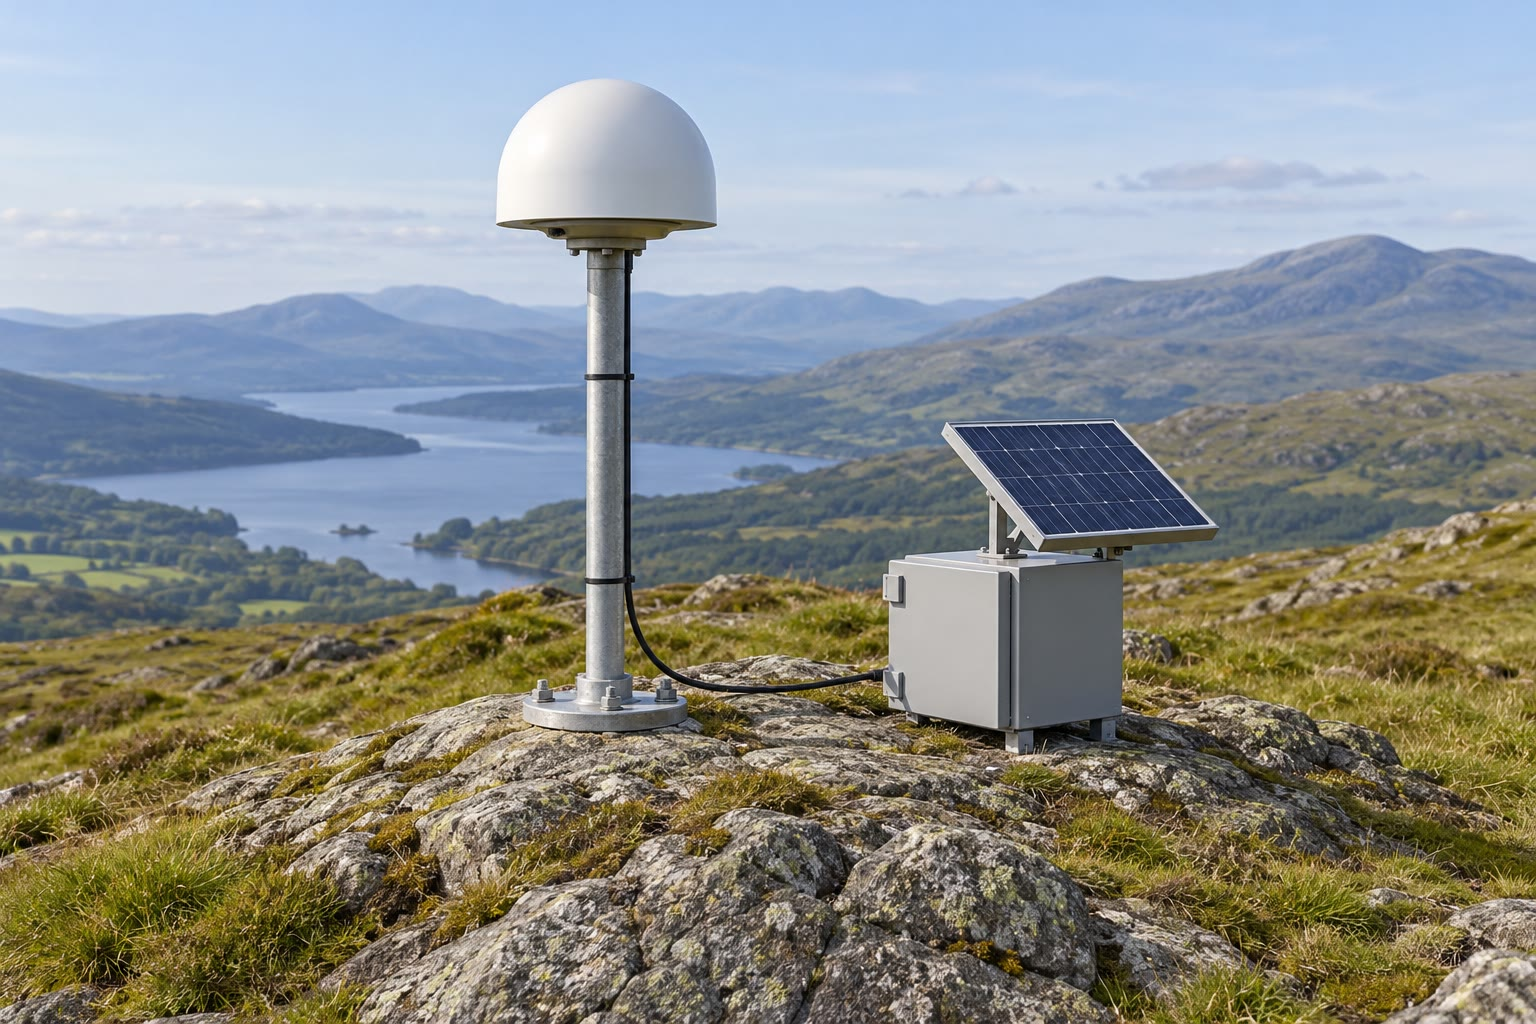
\includegraphics[width=0.55\linewidth]{images/book1/ai/g7-gps-station.jpg}

{\small محطة دائمة لتحديد المواقع: هوائيها مثبت بمسامير في
\omterm{def:g3:stones-pebbles-sand:rock}{الصخر}، فهو يتحرك مع \omterm{def:g7:plate-tectonics:plate}{الصفيحة}.}
\end{omfigure}

\section{تمارين}

\begin{exercise}[$\star$]\label{exo:g7:plate-tectonics:1}
ما \omterm{def:g7:plate-tectonics:continental-drift}{الانجراف القاري}؟ اذكر أنواع الأدلة الأربعة التي استعملها فيغنر
للدفاع عنه.
\end{exercise}

\begin{exercise}[$\star$]\label{exo:g7:plate-tectonics:2}
سمِّ الأنواع الثلاثة \omterm{def:g7:plate-tectonics:plate-boundary}{لحدود الصفائح} وقل، لكل منها، كيف تتحرك
الصفيحتان إحداهما بالنسبة إلى الأخرى.
\end{exercise}

\begin{exercise}[$\star$]\label{exo:g7:plate-tectonics:3}
انظر إلى \omterm{def:g2:drawing-to-map:map}{خريطة} \omterm{def:g4:volcanoes-earthquakes-first-look:earthquake}{الزلازل} \omterm{def:g4:volcanoes-earthquakes-first-look:volcano}{والبراكين}. سمِّ منطقتين من
العالم فيهما \omterm{def:g4:volcanoes-earthquakes-first-look:earthquake}{زلازل} كبيرة كثيرة، \omterm{def:g3:continents-and-oceans:continent}{وقارة} تكاد
لا توجد \omterm{def:g4:volcanoes-earthquakes-first-look:earthquake}{زلازل} في وسطها.
\end{exercise}

\begin{exercise}[$\star$]\label{exo:g7:plate-tectonics:4}
توجد أحافير \emph{الميزوسور}، وهو زاحف صغير عاش في \omterm{def:g2:water-on-earth:salt-fresh}{الماء العذب}،
في البرازيل وفي جنوب إفريقيا. لماذا يُعد ذلك دليلًا على أن
القارتين كانتا ملتحمتين يومًا؟
\end{exercise}

\begin{exercise}[$\star\star$]\label{exo:g7:plate-tectonics:5}
يوجد الفحم في القارة القطبية الجنوبية. ماذا يخبرنا ذلك عن \omterm{def:g5:weather-and-climate:climate}{المناخ} الذي
تكوّن فيه الفحم، وماذا نستنتج عن موقع القارة القطبية الجنوبية
في ذلك الوقت؟
\end{exercise}

\begin{exercise}[$\star\star$]\label{exo:g7:plate-tectonics:6}
قل أي نوع من الحدود يوجد في كل من هذه الأماكن:
ظهرة وسط الأطلسي؛ والأنديز؛ وصدع سان أندرياس؛ والهيمالايا؛
وأخدود شرق إفريقيا.
\end{exercise}

\begin{exercise}[$\star\star$]\label{exo:g7:plate-tectonics:7}
حوّل سرعة مقدارها \qty{2.5}{cm} في السنة إلى كيلومترات في المليون
سنة. ما المسافة التي تتباعدها نقطتان على جانبي الحد
في 60 مليون سنة بهذه السرعة؟
\end{exercise}

\begin{exercise}[$\star\star$]\label{exo:g7:plate-tectonics:8}
بين عامي 1975 و1984 --- أي تسع سنوات --- اتسعت الشقوق القريبة من \omterm{def:g4:volcanoes-earthquakes-first-look:volcano}{بركان} كرافلا
في آيسلندا بنحو \qty{7}{m} في المجموع. ما متوسط
الاتساع في السنة، بالسنتيمترات؟ قارنه بمتوسط سرعة
ظهرة وسط الأطلسي، نحو \qty{2.5}{cm} في السنة، واقترح سببًا لكون
العددين مختلفين إلى هذا الحد.
\end{exercise}

\begin{exercise}[$\star\star$]\label{exo:g7:plate-tectonics:9}
رُفضت نظرية فيغنر عقودًا. ما السؤال الذي لم يستطع أن
يجيب عنه؟ وماذا تغيّر نظرية \omterm{def:g7:plate-tectonics:plate-tectonics}{تكتونية الصفائح} في صورته عن
\omterm{def:g3:continents-and-oceans:continent}{القارات} المتحركة؟
\end{exercise}

\begin{exercise}[$\star\star$]\label{exo:g7:plate-tectonics:10}
انظر إلى المقطع عبر حدين من \omterm{def:g7:plate-tectonics:plate-boundary}{حدود الصفائح}. أين يكون قاع \omterm{def:g2:water-on-earth:ocean}{البحر}
في أعلى \omterm{def:g4:world-physical-map:altitude}{ارتفاع} له، وأين يكون في أعمق نقطة؟ وأين تُصنع \omterm{def:g7:plate-tectonics:plate}{صفيحة} جديدة، وأين
تعود \omterm{def:g7:plate-tectonics:plate}{صفيحة} إلى \omterm{def:g6:inside-the-earth:layers}{الوشاح}؟
\end{exercise}

\begin{exercise}[$\star\star\star$]\label{exo:g7:plate-tectonics:11}
عبر ظهرة شرق \omterm{def:g2:water-on-earth:ocean}{المحيط} الهادئ تتباعد الصفيحتان بنحو \qty{14.2}{cm}
في السنة، وعبر ظهرة شمال الأطلسي بنحو \qty{2.2}{cm} في
السنة. كم مرة تكون ظهرة شرق \omterm{def:g2:water-on-earth:ocean}{المحيط} الهادئ أسرع (قرّب إلى أقرب
عدد صحيح)؟ وكم من الوقت تستغرق كل ظهرة لتفتح \qty{1000}{km} من قاع
\omterm{def:g2:water-on-earth:ocean}{المحيط} الجديد؟
\end{exercise}

\begin{exercise}[$\star\star\star$]\label{exo:g7:plate-tectonics:12}
% ledger: data:usgs-comcat, data:pb2002 (counts in figdata/grade-7/quakes_on_boundaries.py, part bands)
من بين \omterm{def:g4:volcanoes-earthquakes-first-look:earthquake}{الزلازل} التي بلغت قوتها 6 درجات أو أكثر وسُجّلت من 1976 إلى
2025، وعددها 7\,031، وقع 4\,578 على بعد أقل من \qty{100}{km} من خط \omterm{def:g7:plate-tectonics:plate-boundary}{حد
الصفائح} المرسوم على \omterm{def:g2:drawing-to-map:map}{الخريطة}، و6\,472 على بعد أقل من \qty{300}{km}، و6\,786 على بعد أقل
من \qty{500}{km}.
(أ) كم \omterm{def:g4:volcanoes-earthquakes-first-look:earthquake}{زلزالًا} وقع على بعد يتراوح بين \qty{100}{km} و\qty{300}{km} من
الخط؟ (ب) احسب، مقرّبة إلى أقرب عدد صحيح، النسبة المئوية من كل
هذه \omterm{def:g4:volcanoes-earthquakes-first-look:earthquake}{الزلازل} التي وقعت على بعد أقل من \qty{100}{km} من الخط.
(ج) كثير من \omterm{def:g4:volcanoes-earthquakes-first-look:earthquake}{الزلازل} الواقعة على بعد يتراوح بين \qty{100}{km} و\qty{300}{km} من
الخط تقع على الجانب نفسه من خندق محيطي عميق. مستعينًا بما يحدث
عند \omterm{def:g7:plate-tectonics:plate-boundary}{الحد المتقارب}، اشرح لماذا يمكن \omterm{def:g4:volcanoes-earthquakes-first-look:earthquake}{لزلزال} سببه \omterm{def:g7:plate-tectonics:plate-boundary}{حد
صفائح} أن يقع بعيدًا إلى هذا الحد عن الخط المرسوم على \omterm{def:g2:drawing-to-map:map}{الخريطة}.
\end{exercise}

\section{مسألة: انفتاح جنوب الأطلسي}

\begin{problem}[{مسألة نهاية الأسبوع --- قياس محيط على الخريطة
ومعرفة المدة التي استغرقها انفتاحه}]
\label{pb:g7:plate-tectonics:1}
% ledger: data:ne-land, earth:Rmean, data:pb2002, usgs:pangaea-breakup, usgs:atlantic-growth
% (all numbers computed in figdata/grade-7/south_atlantic.py: coasts at 23 S
% at 43.21 W and 14.39 E, 102.4 km per degree, AF-SA full rate 3.43 cm/yr)
على \omterm{def:g2:drawing-to-map:map}{خريطة} لجنوب الأطلسي، يتتبع تلميذ \omterm{def:g6:latitude-longitude:latitude}{دائرة العرض}
\ang{23} جنوبًا. فهي تغادر \omterm{def:g1:landscapes-around-us:water}{ساحل} أمريكا الجنوبية قرب ريو دي
جانيرو، عند \omterm{def:g6:latitude-longitude:longitude}{خط الطول} \ang{43.2} غربًا، وتعبر \omterm{def:g2:water-on-earth:ocean}{المحيط}
وظهرة وسط الأطلسي، وتصل إلى \omterm{def:g1:landscapes-around-us:water}{ساحل} إفريقيا قرب خليج والفيس، عند
\omterm{def:g6:latitude-longitude:longitude}{خط الطول} \ang{14.4} شرقًا. وعلى \omterm{def:g6:latitude-longitude:latitude}{دائرة العرض} هذه، تقيس \omterm{def:g6:latitude-longitude:longitude}{درجة الطول} الواحدة
\qty{102}{km}. وعبر الظهرة، عند هذا \omterm{def:g6:latitude-longitude:latitude}{العرض}، تتباعد صفيحتا أمريكا
الجنوبية وإفريقيا بسرعة \qty{3.4}{cm} في السنة.

\begin{center}
\begin{tikzpicture}
\begin{axis}[axis equal image, xmin=-60, xmax=30, ymin=-42, ymax=12,
  width=0.6\linewidth, tick label style={font=\scriptsize},
  xtick={-60,-40,...,20}, ytick={-40,-20,0},
  xticklabel={$\pgfmathprintnumber{\tick}^\circ$},
  yticklabel={$\pgfmathprintnumber{\tick}^\circ$},
  axis background/.style={fill=omSea}]
\addplot[fill=omLithAlluv, draw=black!45, line width=0.3pt] table {figdata/out/shared-geo-land.dat};
\addplot[omRidge, line width=0.9pt, unbounded coords=jump, restrict x to domain=-45:5] table {figdata/out/shared-geo-school-ridge.dat};
\addplot[omRidge!70!black, line width=0.9pt, unbounded coords=jump, restrict x to domain=-45:5] table {figdata/out/shared-geo-school-transform.dat};
\draw[black, densely dashed, line width=0.7pt] (axis cs:-43.21,-23) -- (axis cs:14.39,-23);
\fill (axis cs:-43.21,-23) circle (1.5pt);
\fill (axis cs:14.39,-23) circle (1.5pt);
\node[font=\scriptsize, below right, inner sep=2pt] at (axis cs:-43.21,-23) {ريو دي جانيرو};
\node[font=\scriptsize, below left, inner sep=2pt] at (axis cs:14.39,-23) {خليج والفيس};
\node[font=\scriptsize, anchor=east, inner sep=1pt] at (axis cs:-16.5,-34) {ظهرة وسط الأطلسي};
\end{axis}
\end{tikzpicture}
\end{center}

\medskip
\noindent\textbf{الجزء الأول --- أدلة التطابق.}
\begin{enumerate}
  \item على \omterm{def:g2:drawing-to-map:map}{خريطة} الأحافير في هذا الفصل، سمِّ الأحافير التي تعبر أشرطتها
        من أمريكا الجنوبية إلى إفريقيا.
  \item لماذا لا يمكن تفسير أحافير \emph{الميزوسور} بحيوان
        سبح من \omterm{def:g3:continents-and-oceans:continent}{قارة} إلى أخرى؟
  \item أي جزء من أمريكا الجنوبية يتطابق مع أي جزء من إفريقيا؟
  \item ما نوع \omterm{def:g7:plate-tectonics:plate-boundary}{حد الصفائح} الذي يمتد في وسط جنوب
        الأطلسي اليوم؟ وكيف تتحرك الصفيحتان هناك؟
\end{enumerate}

\medskip
\noindent\textbf{الجزء الثاني --- قياس المحيط.}
\begin{enumerate}[resume]
  \item كم \omterm{def:g6:latitude-longitude:longitude}{درجة طول} تفصل بين الساحلين على طول
        \omterm{def:g6:latitude-longitude:latitude}{دائرة العرض} \ang{23} جنوبًا؟
  \item ما عرض \omterm{def:g2:water-on-earth:ocean}{المحيط}، بالكيلومترات، على طول \omterm{def:g6:latitude-longitude:latitude}{دائرة العرض}
        هذه؟ قرّب إلى أقرب عشرة كيلومترات.
  \item عند \omterm{def:g3:continents-and-oceans:equator}{خط الاستواء}، تقيس \omterm{def:g6:latitude-longitude:longitude}{درجة الطول} الواحدة \qty{111}{km}.
        فلماذا لا تقيس إلا \qty{102}{km} عند \ang{23} جنوبًا؟
  \item تمتد الظهرة تقريبًا في وسط \omterm{def:g2:water-on-earth:ocean}{المحيط}. فعلى أي بعد تقريبًا
        من الظهرة يقع كل \omterm{def:g1:landscapes-around-us:water}{ساحل}؟
\end{enumerate}

\medskip
\noindent\textbf{الجزء الثالث --- عمر المحيط.}
\begin{enumerate}[resume]
  \item حوّل السرعة التي تتباعد بها الصفيحتان إلى
        كيلومترات في المليون سنة.
  \item لو أن \omterm{def:g2:water-on-earth:ocean}{المحيط} انفتح دائمًا بهذه السرعة، فكم مليون
        سنة كان سيستغرق ليبلغ عرضه الحالي؟ قرّب إلى
        أقرب عشرة ملايين سنة.
  \item يؤرخ الجيولوجيون تفكك \omterm{def:g7:plate-tectonics:supercontinent}{بانجيا} بما بين نحو 225
        و200 مليون سنة مضت، ويقولون إن الأطلسي اتسع خلال
        آخر 100 إلى 200 مليون سنة. هل يتفق جوابك مع ذلك؟
  \item اذكر سببًا واحدًا يجعل العمر الحقيقي لجنوب الأطلسي قد يختلف
        عن العمر الذي وجدته.
\end{enumerate}
\end{problem}
